%%
% !TEX root = main.tex

\RequirePackage[final]{graphicx}
\documentclass[a4paper,fleqn, draft]{cas-sc}



\usepackage{lmodern}
\usepackage[utf8]{inputenc}

%---- PACKAGES
\usepackage{ifdraft}

\usepackage{amssymb}
\usepackage{amsmath}
%\usepackage{mathrsfs}
\usepackage{hyperref}
\usepackage[plain]{fancyref}
\usepackage{subcaption}
\let\labelindent\relax
\usepackage[inline]{enumitem}
\usepackage{xcolor}
\usepackage{tikz}
\usepackage{booktabs}
\usepackage{threeparttable}
\usepackage{multirow}
\usepackage{xspace}
\usepackage[final]{listings}
\usepackage{acronym}
\usepackage{url}
\usepackage{balance}
\usepackage{algorithm}% http://ctan.org/pkg/algorithms
\usepackage{algpseudocode}% http://ctan.org/pkg/algorithmicx
\usepackage[numbers]{natbib}


\usepackage{etoolbox}
\makeatletter
\patchcmd{\@makecaption}
  {\scshape}
  {}
  {}
  {}
\patchcmd{\@makecaption}
  {\\}
  {.\ }
  {}
  {}


\let\refsection\relax
%\usepackage
%  [backend=biber,
%%   natbib=true,
%   style=elsarticle-num-names,
%   maxbibnames=10,
%   minbibnames=5,
%   maxcitenames=1,
%%   giveninits=true,
%   hyperref=true,
%   url=true,
%   defernumbers]{biblatex}
%
%
%%----[ Biber ]----
%\addbibresource[datatype=bibtex]{local.bib}
%\addbibresource[datatype=bibtex]{bib/strings.bib}
%\addbibresource[datatype=bibtex]{bib/general.bib}
%\addbibresource[datatype=bibtex]{bib/compsci.bib}
%\addbibresource[datatype=bibtex]{bib/learning.bib}
%
%\AtEveryBibitem
%  {\clearlist{address}
%   \clearfield{date}
%   \clearfield{doi}
%   \clearfield{eprint}
%   \clearfield{isbn}
%   \clearfield{issn}
%   \clearfield{month}
%   \clearfield{note}
%   \clearfield{pages}
%   \clearlist{location}
%   \clearfield{series}
%   \clearfield{url}
%   \clearname{editor}
%   \ifentrytype{inproceedings}
%     {\clearfield{day}
%      \clearfield{month}
%      \clearfield{volume}}{}}
%
%\DeclareFieldFormat*{title}{\textsl{#1}\isdot}
%\DeclareFieldFormat*{journaltitle}{#1}
%\DeclareFieldFormat*{booktitle}{#1}
%
%\renewbibmacro{in:}{} % supress 'In: ' form
%
%\DeclareSourcemap
% {\maps[datatype=bibtex,overwrite]
%   {% Tag entries (through keywords)
%    \map
%      {\step[fieldsource=booktitle,
%       match=\regexp{[Pp]roceedings}, replace={Proc.}]}
%    \map
%      {\step[fieldsource=booktitle,
%       match=\regexp{[Ii]nternational}, replace={Intl.}]}
%   \map
%      {\step[fieldsource=booktitle,
%       match=\regexp{[Cc]onference}, replace={Conf.}]}
%    \map
%      {\step[fieldsource=booktitle,
%       match=\regexp{[Ss]ymposium}, replace={Symp.}]}
%    \map
%      {\step[fieldsource=journal,
%       match=\regexp{[Jj]ournal}, replace={Jour.}]}
%    \map
%      {\step[fieldsource=journal,
%       match=\regexp{[Tt]ransactions}, replace={Trans.}]}
%	\map
%      {\step[fieldsource=journal,
%       match=\regexp{[Aa]nnals}, replace={Ann.}]}
%	\map
%      {\step[fieldsource=journal,
%       match=\regexp{[Ss]oftware}, replace={Soft.}]}
%	\map
%      {\step[fieldsource=journal,
%       match=\regexp{[Ee]ngineering}, replace={Eng.}]}
%    \map
%      {\step[fieldsource=booktitle,
%       match=\regexp{[Pp]roceedings\s+of\s+the.+[Ee]uropean\s+[Cc]onference\s+in}, replace={European Conf. in}]}
%    \map
%      {\step[fieldsource=booktitle,
%       match=\regexp{In\s+[Pp]roceedings\s+of\s+the\s+[Ss]ymposium\s+on}, replace={Symp. on}]}
%     \map
%      {\step[fieldsource=publisher,
%       match=\regexp{[Aa]ssociation\s+for\s+[Cc]omputing\s+[Mm]achinery\s}, replace={ACM}]}
%     \map
%      {\step[fieldsource=booktitle,
%       match=\regexp{[Pp]roceedings\s+of\s+the\s+[Ii]nternational\s+[Cc]onference\s+on}, replace={Intl. Conf. on}]}
%    \map
%      {\step[fieldsource=booktitle,
%       match=\regexp{[Pp]roceedings\s+of\s+the\s+[Ii]nternational\s+[Ww]orkshop\s+on}, replace={Intl. Workshop on}]}}}



%color
\definecolor{OliveGreen}{rgb}{0,0.6,0.3}

%References
%% Listings
\def\fref{\Fref} % treat all \frefs as \Frefs
\renewcommand{\lstlistingname}{Snippet}
\newcommand*{\fancyreflstlabelprefix}{lst}
\newcommand*{\Freflstname}{\lstlistingname}
\newcommand*{\freflstname}{\MakeLowercase{\lstlistingname}}
\Frefformat{vario}{\fancyreflstlabelprefix}%
  {\Freflstname\fancyrefdefaultspacing#1#3}
\frefformat{vario}{\fancyreflstlabelprefix}%
  {\freflstname\fancyrefdefaultspacing#1#3}
\Frefformat{plain}{\fancyreflstlabelprefix}%
  {\Freflstname\fancyrefdefaultspacing#1}
\frefformat{plain}{\fancyreflstlabelprefix}%
  {\freflstname\fancyrefdefaultspacing#1}

\renewcommand{\tablename}{Table}  
\renewcommand{\figurename}{Figure}  
  
% ln delimiter
\newcommand*{\fancyreflnlabelprefix}{ln}
\newcommand*{\Freflnname}{Line}
\newcommand*{\freflnname}{\MakeLowercase{\Freflnname}}
\Frefformat{vario}{\fancyreflnlabelprefix}%
  {\Freflnname\fancyrefdefaultspacing#1#3}
\frefformat{vario}{\fancyreflnlabelprefix}%
  {\freflnname\fancyrefdefaultspacing#1#3}
\Frefformat{plain}{\fancyreflnlabelprefix}%
  {\Freflnname\fancyrefdefaultspacing#1}
\frefformat{plain}{\fancyreflnlabelprefix}%
  {\freflnname\fancyrefdefaultspacing#1}    

%def delimiter
\newcommand*{\fancyrefdeflabelprefix}{def}
\newcommand*{\Frefdefname}{Definition}
\newcommand*{\frefdefname}{\MakeLowercase{\Frefdefname}}
\Frefformat{vario}{\fancyrefdeflabelprefix}%
  {\Frefdefname\fancyrefdefaultspacing#1#3}
\frefformat{vario}{\fancyrefdeflabelprefix}%
  {\frefdefname\fancyrefdefaultspacing#1#3}
\Frefformat{plain}{\fancyrefdeflabelprefix}%
  {\Frefdefname\fancyrefdefaultspacing#1}
\frefformat{plain}{\fancyrefdeflabelprefix}%
  {\frefdefname\fancyrefdefaultspacing#1}    
  
%theorem delimiter
\newcommand*{\fancyreftheolabelprefix}{theo}
\newcommand*{\Freftheoname}{Theorem}
\newcommand*{\freftheoname}{\MakeLowercase{\Freftheoname}}
\Frefformat{vario}{\fancyreftheolabelprefix}%
  {\Freftheoname\fancyrefdefaultspacing#1#3}
\frefformat{vario}{\fancyreftheolabelprefix}%
  {\freftheoname\fancyrefdefaultspacing#1#3}
\Frefformat{plain}{\fancyreftheolabelprefix}%
  {\Freftheoname\fancyrefdefaultspacing#1}
\frefformat{plain}{\fancyreftheolabelprefix}%
  {\freftheoname\fancyrefdefaultspacing#1}    

%Proposition delimiter
\newcommand*{\fancyrefproplabelprefix}{prop}
\newcommand*{\Frefpropname}{Proposition}
\newcommand*{\frefpropname}{\MakeLowercase{\Frefpropname}}
\Frefformat{vario}{\fancyrefproplabelprefix}%
  {\Frefpropname\fancyrefdefaultspacing#1#3}
\frefformat{vario}{\fancyrefproplabelprefix}%
  {\frefpropname\fancyrefdefaultspacing#1#3}
\Frefformat{plain}{\fancyrefproplabelprefix}%
  {\Frefpropname\fancyrefdefaultspacing#1}
\frefformat{plain}{\fancyrefproplabelprefix}%
  {\frefpropname\fancyrefdefaultspacing#1}    
  
  
%Code environment definition
\lstset{%
  basicstyle=\footnotesize\ttfamily,
  aboveskip=0\baselineskip,
  belowskip=0\baselineskip,
  commentstyle=\scriptsize\itshape,
  keywordstyle=\ttfamily\bfseries,
  breaklines,
  numberblanklines=false,
  numberstyle=\tiny\color{gray}, 
  commentstyle=\color{gray},
  numbersep=0pt,
  escapechar=`,  
  numberbychapter=false}
  
\lstdefinestyle{floating}
 {frame=lines,
  float=hptb,
  captionpos=b,
  abovecaptionskip=-0pt}

% python listings
\lstdefinestyle{py}
 {language=Python,
  showstringspaces=false,
  tabsize=2,
  style=floating,
  belowskip=-0\baselineskip,
  aboveskip=-0\baselineskip,
  keywords=[2]{def, for, while, if, else, return, self},
%  deletekeywords={len, max, range},
  keywordstyle=[2]\ttfamily\bfseries,
  keywords=[1]{breakpoint,n,p,pp,s,c,step_back,back_to,variables,sticky,args,setvar,unt,b,w,u,d,help,q},
  keywordstyle=[1]\ttfamily\bfseries\color{blue},
  deletekeywords={len,max,range},
}

%context traits environment    
 \lstnewenvironment{python}[1][]
 {\lstset{style=py,#1}}{}  

 % Context Traits in line source-code
\newcommand{\spy}[1]{\lstinline[style=py]{#1}}


%%Boxes
\usepackage[many]{tcolorbox} 
\usepackage{setspace} 

\setlength\parindent{0pt}   % killing indentation for all the text
\setstretch{1}            % setting line spacing to 1.3
%\setlength\columnsep{0.1in} % setting length of column separator
\pagestyle{empty}           % setting pagestyle to be empty


\definecolor{main}{HTML}{5989cf}    % setting main color to be used
\definecolor{sub}{HTML}{cde4ff}     % setting sub color to be used

\tcbset{
    sharp corners,
    colback = white,
    before skip = 0.1cm,    % add extra space before the box
    after skip = 0.2cm      % add extra space after the box
} 

\newtcolorbox{highlight}{
    colback = sub, 
    colframe = main, 
    boxrule = 0pt, 
    leftrule = 3pt % left rule weight}
}

%----[ Figures ]---
%\addtolength{\intextsep}{-1mm}

%%captions
%\addtolength{\abovecaptionskip}{-0mm}
%\addtolength{\belowcaptionskip}{-0mm}
%\captionsetup[figure]{aboveskip=-0ex,belowskip-0ex}
%\captionsetup[table]{aboveskip=-0ex,belowskip-0ex}
%\captionsetup[lstlisting]{aboveskip=-1ex,belowskip=-1ex}

%DPN
%\usepackage[version=0.96]{pgf}
%\usetikzlibrary{arrows, shapes, backgrounds}
%\usetikzlibrary{decorations.pathreplacing}
%\usetikzlibrary{shapes.misc}
%\usetikzlibrary{petri}

%% Petri nets
\tikzstyle{place}=[circle,thick,draw=black!75,minimum size=5mm]
\tikzstyle{iplace}=[circle,dashed,thick,draw=black!75,minimum size=5mm]
\tikzstyle{itransition}=[rectangle,draw,thick,fill=black,minimum size=1mm]
\tikzstyle{etransition}=[rectangle,draw,thick,minimum size=1mm]
\tikzstyle{ctransition}=[rectangle,draw,color=black!45,thick,fill=black!45,minimum size=1mm]

\tikzstyle{dpn}=
 [node distance=1.3cm, >=stealth', bend angle=45, auto,
  font=\fontsize{8}{8}\selectfont]

%----[ Commands ]---
%Latins
\newcommand{\eg}{\emph{e.g.,}\xspace}
\newcommand{\ie}{\emph{i.e.,}\xspace}
\newcommand{\cf}{\emph{cf.}\xspace}

\newcommand{\ctx}[1]{\texttt{\textsc{#1}}}

%petri
\newcommand{\enabled}[2]{$#1[#2\rangle$}
%names
\newcommand{\flik}{\textsc{Flik}\xspace}

%comments
% xcolor
\definecolor{author}{rgb}{.5, .5, .5}
\definecolor{comment}{rgb}{.1, .0, .9}
\definecolor{note}{rgb}{.9, .4, .0}
\definecolor{idea}{rgb}{.1, .7, .0}
\definecolor{missing}{rgb}{.9, .1, .0}


\newcommand{\authorcomment}[3][comment]
  {\ifdraft{\noindent
      \fbox{\footnotesize\textcolor{author}{\textsc{#2}}}
      \textcolor{#1}{\textsl{#3}}}{}}

% $Id: acronyms.tex  $
% !TEX root = main.tex

\acrodef{RL}{Reinforcement Learning}
\acrodef{AI}{Artificial Intelligence}
\acrodef{ML}{Machine Learning}
\acrodef{GDB}{GNU Debugger}
\acrodef{IDE}{Integrated Development Environment}
\acrodef{API}{Application Programming Interface}
\acrodef{DDD}{Data-Display Debugger}
\acrodef{PDB}{Python Debugger}
\acrodef{GUI}{Graphical User Interface}
\acrodef{RevPDB}{Reverse Python Debugger}
\acrodef{UDB}{Undo Debugger}
\acrodef{Vizarel}{A Tool for Interactive Visualization of Reinforcement Learning}
\acrodef{MDP}{Markov Decision Process}
\acrodef{TD}{Temporal-Difference}

%---[ Acronyms Plurals Special Forms] ---


%\newcommand{\acResetNonTrivial}
  

%\acResetNonTrivial
{\acresetall
   \acused{CPU}
   \acused{VAR}
   \acused{AST}
   \acused{API}
   \acused{LAN}
   \acused{SMT}
   \acused{GUI}}


\endinput

%Space squeezing
\let\orig@figure\figure
\renewcommand*{\figure}[1][]{\orig@figure[#1]\vspace{-1ex}} % before
\let\orig@endfigure\endfigure
\renewcommand*{\endfigure}{\vspace{-1.5ex}\orig@endfigure} % after

\let\orig@endlstlisting\endlstlisting
\renewcommand*{\endlstlisting}{\vspace{-3ex}\orig@endlstlisting} % after

% Squeeze captions
\usepackage{caption}
\captionsetup[figure]{aboveskip=0.0em,belowskip=-0em}
\captionsetup[table]{aboveskip=0em,belowskip=-0em}



\makeatother
% $Id: acronyms.tex  $
% !TEX root = main.tex

\acrodef{RL}{Reinforcement Learning}
\acrodef{AI}{Artificial Intelligence}
\acrodef{ML}{Machine Learning}
\acrodef{GDB}{GNU Debugger}
\acrodef{IDE}{Integrated Development Environment}
\acrodef{API}{Application Programming Interface}
\acrodef{DDD}{Data-Display Debugger}
\acrodef{PDB}{Python Debugger}
\acrodef{GUI}{Graphical User Interface}
\acrodef{RevPDB}{Reverse Python Debugger}
\acrodef{UDB}{Undo Debugger}
\acrodef{Vizarel}{A Tool for Interactive Visualization of Reinforcement Learning}
\acrodef{MDP}{Markov Decision Process}
\acrodef{TD}{Temporal-Difference}

%---[ Acronyms Plurals Special Forms] ---


%\newcommand{\acResetNonTrivial}
  

%\acResetNonTrivial
{\acresetall
   \acused{CPU}
   \acused{VAR}
   \acused{AST}
   \acused{API}
   \acused{LAN}
   \acused{SMT}
   \acused{GUI}}


\endinput


\begin{document}
 
% Short title
\shorttitle{Flik}    

% Short author
\shortauthors{L. Rodriguez et al.}  

% Main title of the paper
\title[mode = title]{Flik: A Back-in-time Debugger for Reinforcement Learning Programs}  

% Title footnote mark
% eg: \tnotemark[1]
%\tnotemark[1] 

% Title footnote 1.
% eg: \tnotetext[1]{Title footnote text}
%\tnotetext[1]{} 

% First author
%
% Options: Use if required
% eg: \author[1,3]{Author Name}[type=editor,
%       style=chinese,
%       auid=000,
%       bioid=1,
%       prefix=Sir,
%       orcid=0000-0000-0000-0000,
%       facebook=<facebook id>,
%       twitter=<twitter id>,
%       linkedin=<linkedin id>,
%       gplus=<gplus id>]

\author[1]{Laura {Rodriguez}}[orcid=0009-0000-9715-0475]
\ead{la.rodriguez@uniandes.edu.co}

\author[1]{Mario {Linares-V\'asquez}}[orcid=0000-0003-0161-2888]
\ead{m.linarev@uniandes.edu.co}

\author[2]{{Ivana} {Dusparic}}[orcid=0000-0003-0621-5400]
\ead{ivana.dusparic@tcd.ie}

\author[1]{{Nicol\'as} {Cardozo}}[orcid=0000-0002-1094-9952]
\ead{n.cardozo@uniandes.edu.co}
\cormark[1]

% Address/affiliation
\affiliation[1]{organization={Department of Systems and Computing Engineering, Universidad de los Andes}, 
	city={Bogota}, 
	country={Colombia}}

\affiliation[2]{organization={School of Computer Science and Statistics, Trinity College Dublin}, 		city={Dublin}, 
	country={Ireland}}


% Corresponding author text
\cortext[1]{Corresponding author}



% For a title note without a number/mark
%\nonumnote{}

% Here goes the abstract
\begin{abstract}
%Why
\textbf{Purpose:} \ac{RL}-based programs' have a high-level of complexity due to the size and 
conditions of the environment, and agents' interaction with it. Developers face challenges  
understanding the behavior of \ac{RL} agents and identifying bugs, and their cause, within the 
program execution. This problem is particularly challenging for bugs in which the program runs 
without errors, but the execution does not present an appropriate agent behavior.
%What
\textbf{Method:} To address this problem, we propose \flik, a back-in-time debugger for \ac{RL} 
programs. \flik is a console-based debugger that allows developers to interact with 
the program during execution, inspect the internal state of the agent, and modify 
its behavior in real-time. Changes to the agent generate alternative execution paths. Based on such 
execution path, developers can more easily identify bugs in their programs.
\textbf{Results:} We evaluate the usability and usefulness of \flik in identifying and helping to solve 
bugs by means of a user evaluation in which 27 developers interacted and solve bugs in three 
different \ac{RL}  programs. Our results show a positive response to \flik, highlighting that the 
debugger is useful in identifying the kinds of bugs that commonly arise in \ac{RL} programs. 
\textbf{Conclusion:} 
With the advent of \ac{RL} programs, software engineering and analysis tools are need to help 
assure their correct execution. This work presents a back-in-time debugger with functionality to 
updated agents' state during their execution to be able to observe behavioral changes immediately, 
without having to re-execute the entire agent. The debugger proved useful through a user study 
confirming the importance of such tools.
\end{abstract}

% Use if graphical abstract is present
%\begin{graphicalabstract}
%\includegraphics{}
%\end{graphicalabstract}

% Research highlights
\begin{highlights}
\item Presentation of a first debugger for Reinforcement learning programs, based on back-in-time debugging capabilities.
\item Full implementation of a text/console-based debugger with the capability to: step through the code; observe variables' state; modify variables' state during execution to branch different execution paths; and step back in the execution restoring the state and execution context (stack instructions), again enabling teh possibility to branch execution with different contexts.. 
\item Empirical study with 27 participants, developed to evaluate the usefulness and usability of the debugger in identifying bugs in three different Q-learning programs.
\end{highlights}


% Keywords
% Each keyword is seperated by \sep
\begin{keywords}
Debuggers \sep
Back-in-time \sep 
Reinforcement Learning \sep 
Empirical Study
\end{keywords}


\maketitle              % typeset the header of the contribution

% $Id: problem.tex 
% !TEX root = ../main.tex

\section{Introduction}
\label{sec:problem}

\section{Reinforcement Learning}

% Section: Explanation of RL
% common bugs in RL programs.
Before starting with the problem let us understand a how \ac{RL} works and why it is  
important to properly develop in nowadays.
\ac{RL} algorithms were introduced by~\citet{sutton98}, the idea behind these 
algorithms is to learn the optimal policy (a set of actions) through the interaction 
with the environment. \ac{RL} uses an agent that learns the value function for a given policy 
through interaction with the environment to predict an optimal solution and based on the value 
function, it continuously develops and learns the optimal policy. One of the most common algorithms
in \ac{RL} is Q-learning~\cite{8836506}, which uses an off-policy control that separates the deferral 
policy from the learning policy and updates the action selection using the Bellman optimal equations
and the e-greed policy. As with normal \ac{RL} algorithms, Q-learning involves an agent, a set of states
$S_j$ and a set of actions $A$. By performing an action $a\in A$ at state $s \in S$, the agent 
transitions from $s$ to a new state $s' \in S$, which will give a $reward$ $r$ to the agent. 
The goal of the agent is to maximize its 
total reward. The following \fref{lst:qlearning} 
of code is the usual pseudo algorithm for 
Q-learning off policy algorithms~\cite{Sutton1998}.

\begin{algorithm}
\caption{Q-Learning Algorithm}\label{lst:qlearning}
\begin{algorithmic}
\Require An environment with states $S$, actions $A$, and reward function $R(s, a)$
\Require A learning rate $\alpha \in [0, 1]$
\Require A discount factor $\gamma \in [0, 1]$
\Require Exploration strategy (e.g., $\epsilon$-greedy)
\State Initialize Q-table $Q(s, a) \gets 0$ for all $s \in S$, $a \in A$
\For{each episode}
    \State Initialize the starting state $s_0$
    \For{each time step in the episode}
        \If{exploration step}
            \State Choose an action $a$ using the exploration strategy (e.g., $\epsilon$-greedy)
        \Else
            \State Choose an action $a$ based on the current Q-values: $a = \arg\max\_a Q(s, a)$
        \EndIf
        \State Take action $a$, observe reward $r$ and next state $s'$
        \State Update Q-value: 
        \[
        Q(s, a) \gets Q(s, a) + \alpha \left( r + \gamma \max_{a'} Q(s', a')\right)
        \]
        \State Set $s \gets s'$
    \EndFor
\EndFor
\end{algorithmic}
\end{algorithm}

\ac{RL} programs have a wide range of applications, \citet{8836506} presents a comparison table with some 
\ac{RL} applications. Nevertheless, some of the most them could be: from control of industrial process~\cite{8169685} (improving 
the performance of the on-line learning control system or optimizing temperature control and power consumption),
to computer networking~\cite{AlRawi2013ApplicationOR} (improving adaptability of Wireless Sensor Networks to changing situations and eliminating 
the need for system redesign) and robotics~\cite{zhang2015visionbaseddeepreinforcementlearning} (by providing frameworks and toolkits for designing sophisticated 
behavioral aspects). 

When developing \ac{RL} programs, issues arise in the application logic like wrong value for the
learning rate or wrong definition of the rewards. This requires a call for the developer for stronger frameworks in which 
the implementation (and implementation experience) could improve for \ac{RL} applications. One possible first step 
is in the creation of tools to help developers understand and analyze their programs and their behavior.

\section{Problem}

\ac{RL} programs (like \ac{ML} programs), 
have a significant limitation: they function as a black box. 
This means that it is impossible to know how the programs reached a decision. This poses 
a problem in many fields, as it often becomes difficult to identify why a model 
fails to converge or why it does not reach an optimal or expected solution as 
anticipated by the developer. In the case of \ac{RL}, this issue is particularly 
pronounced because it is challenging to determine whether the agent is learning 
correctly or if it is learning an inappropriate policy.

Furthermore, \ac{RL} programs are notoriously difficult to debug due to the extensive 
training periods they require, which demand substantial computational power. This 
complexity makes it incredibly challenging to locate errors, even when using a 
debugger for standard programs. Traditional debugging tools are often inadequate 
for tracing the issues in \ac{RL} due to the intricate and prolonged nature of the 
training processes. 
% This is because \ac{RL} programs have an added difficulty: they 
% operate with a different execution cycle compared to traditional programs.

In conventional software, the execution flow is typically linear and predictable, 
allowing developers to trace and debug step-by-step with relative ease. However, 
\ac{RL} programs involve a continuous loop of learning and adaptation, where an agent 
interacts with an environment, receives feedback in the form of rewards or 
penalties, and adjusts its actions accordingly. This cyclical nature makes the 
process much more complex and less transparent.

In \ac{RL}, each decision and its subsequent outcome can affect future decisions, 
creating a dynamic and interdependent series of events. This complexity is 
compounded by the often stochastic nature of environments, where the same action 
can lead to different results in different contexts or iterations. As a result, 
understanding and debugging \ac{RL} programs require not only tracking individual 
decisions but also understanding the long-term effects and patterns that emerge 
over many iterations.

Moreover, the need for substantial computational resources and extended training 
periods adds to the challenge. The iterative process can take hours, days, or 
even weeks, making it impractical to simply restart the training from scratch 
each time an error is detected. The aforementioned problems and characteristics
of the execution in \ac{RL} posits the need for advanced tools and methods 
for visualizing the agent's behavior, monitoring its learning progress, and 
pinpointing issues without having to re-run lengthy training sessions.

Therefore, the distinct execution cycle of \ac{RL} programs introduces unique 
challenges that demand specialized debugging and visualization tools to ensure 
effective development and deployment. Addressing these challenges is crucial 
for advancing the field of reinforcement learning and making its applications 
more reliable and interpretable.

Therefore, there is a pressing need for a tool that allows for the visualization 
of an \ac{RL} agent's behavior and facilitates appropriate debugging of \ac{RL} the programs. 
Such a tool would significantly enhance the transparency and interpretability 
of \ac{RL} models, making it easier for developers to understand, refine, and correct 
the learning process. This is a gap in the current literature, and addressing it 
is the focus of this work.

The structure of the paper is as follows: Chapter 2 an introduction to debuggers (\fref{sec:deb}),
it also provides a comprehensive review of the state of the art in the field of back in 
time debuggers in any programming language (\fref{sec:other}), in python (\fref{sec:py})
and in \ac{RL} (\fref{sec:ai}). Chapter 3 presents the proposed solution, \flik, 
a back in time debugger for \ac{RL} programs. Chapter 4 presents the evaluation of the tool,
the three proposed exercises (\fref{sec:grid-eval}, \fref{sec:rooms-eval} and 
\fref{sec:cars-eval}) and the evaluation setup (\fref{sec:evaluation}). Chapter 5 presents the 
results of the evaluation and the feedback from the participants, divided in the 
three main parts of the survey: general results (\fref{sec:general-knowledge}), tasks 
results (\fref{sec:tasks-results}) and usability results (\fref{sec:usability}). It also adds 
a final part for the discussion of the results (\fref{sec:discussion}). 
Finally, \fref{sec:conclusion} presents the conclusion 
and avenues for future work.


\endinput


% $Id: state_of_the_art.tex 
% !TEX root = ../main.tex

\section{State of the Art}
\label{sec:state_of_the_art}

This section presents the state of the art with respect to four main dimensions, covering the definition 
of debuggers, the main debuggers in other programming languages, existing Python debuggers, and, 
finally, debuggers for \ac{AI} programs in general, and \ac{RL} specifically.


%%
\subsection{What is a Debugger?}
\label{sec:deb}

A software bug is defined as erroneous behavior observed during a program's execution, causes the 
program to crash or produce incorrect results. Bugs are common in software development, and can 
be caused by many factors, such as incorrect program logic, incorrect syntax used, or incorrect data. 
Bugs can be difficult to identify and fix, especially in large and complex programs. In this work we 
focus in run-time errors, in which programs compile, but present an abnormal behavior caused by 
incorrect program logic. Debugging is the process of finding and reducing the number of 
bugs or defects in a program~\cite{hindriks12}. In practical terms, debugging is defined as the 
activity that comes after testing, when developers identify an (execution/behavioral) error and modify
the program to fix the bug~\cite{mccauley08}. 

There are several principles that guide the debugging process, these principles are explained in the 
book the Art of debugging with \ac{GDB}, \ac{DDD}, and Eclipse~\cite{matloff08}. The fundamental 
principle that drives the essence of debugging is the \emph{Principle of Confirmation}: fixing a 
program with bugs is a process of confirming that the things you believe to be true are actually true in 
your code~\cite{matloff08}. This means that when you find that those assumptions are not true, you 
have find the bug, and fix it.

A classic debugging technique is adding traces in your code in terms of printing the values of several 
variables as the program is executed. However, this is not an efficient or scalable way to debug a 
program, reason why debuggers exist. A debugger is a tool that allows developers to inspect the 
state of a program while it is running, and to control its execution. Debuggers are essential tools for 
software development, as they help developers to identify and fix bugs in their programs. There are 
many types of debuggers, each with its own set of features and capabilities, but usually the main 
operations offered by debuggers~\cite{matloff08} are:

\begin{itemize}
    \item Stepping through code: where developers can run the program stepping at each of the 
    instructions individually, or step for a number of instructions, stopping at a predefined program 
    instruction or  \emph{breakpoint}. Additionally, it is possible to step into the execution of a particular 
    instruction, to observe its behavior in detail. 
    \item Inspecting variables: where developers can inspect the current values of variables in the 
    program. This is helpful to understand the change in state, possibly giving clues on possible causes 
    of the undesired behavior.
    \item Changing the program state: developers can change the values of variables in the program. 
    This is useful to test different scenarios during the program execution. However useful, this feature 
    is seldomly available across debuggers.
\end{itemize}

In summary, a debugger is a tool that allows developers to inspect the state of a program, control 
its execution, and possibly change its state. Driven by these operations, debuggers are essential 
tools for software development, as they help developers to identify and fix bugs in their programs. 
In this work, we want to understand \ac{RL} programs; to understand agents' behavior and 
create higher quality code. Our solution proposes a debugger with all three aforementioned features
to achieve such behavior.


%%
\subsection{Debuggers for other programming languages}
\label{sec:other}

We now turn our attention to the state of the art in debugging tools available for different 
programming languages. There are many debugging tools available for different programming 
languages, each with its own set of features and capabilities, most of them integrated with IDEs as
built-in debugging tools that allow developers to inspect programs' behavior during their execution. 
However, there are also standalone debugging tools that can be used with different 
programming languages, and that offer more advanced features and capabilities than the 
built-in debugging tools of IDEs. 

Some of the most popular debugging tools include \ac{GDB}~\cite{stallman11}, 
which stands for GNU Project Debugger and is a powerful 
debugging tool for C and C++ (although it also supports other programming languages,
like Ada, Go, or Rust). GDB helps developers to inspect the internals of C programs while 
they are executing. \ac{GDB} works on binary executable files produced during compilation. During 
execution, \ac{GDB} allows developers to observe exactly what happens when a program 
crashes. \ac{GDB} consists of three major subsystems~\cite{stallman11}. 
\begin{enumerate*}[label=(\arabic*)] 
\item The user interface subsystems, consists of several actual interfaces, plus their supporting code. 
\item The symbol handling subsystem, consists of object file readers, debugging info interpreters, 
symbol table management, source language expression parsing, and type and value printing. 
\item The target system handling, consists of execution control, stack frame analysis, and 
physical target manipulation.
\end{enumerate*}

DeloreanJs~\cite{leger23} is a back-in-time debugger for JavaScript programs. The value of 
back-in-time debuggers is the possibility to rewinding execution to a specific point, allowing the 
possibility for developers to, for instance, test different variable values within the same execution 
context, to better understand errors or explore hypothetical scenarios in the program's execution 
evolution~\cite{hofer06,lienhard09}. DeloreanJs has three main features: the ability to navigate 
through an execution history, modify values of a variable, and resume execution from a timepoint (a 
specific execution point in the past)~\cite{leger23}. DeloreanJS extends continuations with static 
analysis functionalities to capture the current program state, and store the (history of) variable's 
values. There are several other debuggers for Javascript, must of them based on the use of 
breakpoints, in which variables cannot be modified to resume current execution with the new values, 
similar to the behavior offered in \ac{GDB}.

We note the functionality to go back in time, observe the program's state at a previous moment and 
execute a new timeline with the new values, offered by DeloreanJS, and in general back-in-time 
debuggers, is desirable in the context of \ac{RL} programs. Therefore we use  back-in-time 
debuggers, and DeloreanJS, as a reference to create our debugger for \ac{RL} programs.


%%
\subsection{Python debuggers}
\label{sec:py}

Given that  most \ac{RL} programs are written in Python, we pay special attention to existing 
debuggers for Python. There are several Python debuggers available. We focus on those debuggers
that have support for the features required to debug \ac{RL} programs, such as: the ability to navigate 
through an execution history (like a time traveling debugger), and the ability to modify the values
of variables and resume the execution from a specific point in time.

% PDB
The \ac{PDB}~\cite{python-pdb} debugger is the built-in Python Debugger in CPython~\cite{shaw21} 
(the standard Python bytecode interpreter), implemented by several IDEs that provide a missing 
visual interface. \ac{PDB} is a powerful interactive source code debugger for Python programs, 
implemented as a module that can be used in Python scripts. \ac{PDB} provides a command-line 
interface for debugging Python programs, allows developers to define breakpoints, step through 
program instructions, inspect variables, and evaluate expressions. Additionally, \ac{PDB} provides 
a post-mortem debugging feature that allows developers to debug a program after it has crashed. 
However, \ac{PDB} does not have the ability to navigate through the execution history of a program, 
modify values of variables, or resume execution from a specific point in time, which are the features 
we are looking for in our solution. 

% PuDB
PuDB~\cite{pudb} is a full-screen, console-based visual debugger for Python. PuDB allows 
developers to set breakpoints, step through code, inspect variables, and evaluate expressions. 
Similar to \ac{PDB}, PuDB also provides a post-mortem debugging feature that allows developers to 
debug a program after it has crashed. However, PuDB does not have the ability to navigate through 
a program's execution history, modify values of variables, or resume execution from a specific point 
in time. Nevertheless, the history navigation feature can be simulated placing breakpoints in the 
code, and restarting the execution until the breakpoint is reached. The UI makes it possible to go 
through the code and see the variables and the stack trace in a user-friendly fashoin.

% PyTrace
PyTrace~\cite{pytrace} is a time travel recorder/analyzer for Python. PyTrace records code execution, 
variables and stack frames. It has a UI that allows developers to navigate through the code, 
see the variables and the stack trace, and it is very user-friendly. However, PyTrace is not 
a full-featured debugger, as it does not allow you to change the values of variables, or do 
any other operation available to debuggers. PyTrace works as a tool to understand the behavior of 
a program, moving backward and fordward through a recorded execution (again in a single execution 
path),  with different different graphs to see the state of your variables at a moment in time.

% RevPDB
\ac{RevPDB}~\cite{revdeb} is a reverse debugger for Python programs, RevPDB is an extension of 
\ac{PDB} built on top of the PyPy interpreter, allowing developers to go forward and backward in time. 
However, RevPDB is not a full-featured debugger nor it has a user-friendly UI, as it is a proof of 
concept of the time traveling features, and it is not currently maintained.


% UDB
\ac{UDB}~\cite{udb} is a proprietary debugger, developed by the Company Undo, for Python 
programs that allows developers to navigate through time and inspect the state of the program at a 
previous moment in time. \ac{UDB} works on the principle of first recording 
a program while it is running normally, and then replaying the execution while allowing the 
developer to navigate and inspect the program's state at different points in time. \ac{UDB} works at 
the process level, rewinding and replaying the state of the entire process. Technically, 
\ac{UDB} does allow new code paths to be executed at replay-time, but all execution replays are 
isolated.

\fref{tab:python-debuggers} shows a comparative summary of existing Python debuggers, the 
features they offer. 

\begin{table}[hptb]
  \centering
  \resizebox{\columnwidth}{!}{%
\begin{tabular}{c|lllll}
\textbf{Features}               & \multicolumn{1}{c}{\textbf{PDB}}                                                         & \multicolumn{1}{c}{\textbf{PuDB}}                                                                               & \multicolumn{1}{c}{\textbf{PyTrace}}                                           & \multicolumn{1}{c}{\textbf{RevPDB}}                                                   & \multicolumn{1}{c}{\textbf{UDB}}                                                                                                          \\ \toprule
\textbf{Description}            & \begin{tabular}[c]{@{}l@{}}Terminal debugger based\\ on CPython interpreter\end{tabular} & \begin{tabular}[c]{@{}l@{}}UI Debugger that extends\\ PDB debugger\end{tabular}                                 & Post mortem debugger                                                           & \begin{tabular}[c]{@{}l@{}}Terminal debugger based\\ on PyPy interpreter\end{tabular} & \begin{tabular}[c]{@{}l@{}}Not open source.\\ Has functionalities for \\  back in time debugging\\ for pdb.\end{tabular} \\
\textbf{Stepping}               & It allows stepping                                                                       & It allows stepping                                                                                              & It allows stepping                                                             & It allows stepping                                                                    & It allows stepping                                                                                                                        \\
\textbf{Breakpoints}            & It allows breakpoints                                                                    & It allows breakpoints                                                                                           & Does not allow breakpoints                                                      &                                                                                       & It allows breakpoints                                                                                                                     \\
\textbf{Stepping back}          & \begin{tabular}[c]{@{}l@{}}It can be simulated using \\ jumps through time\end{tabular}  & \begin{tabular}[c]{@{}l@{}}It can be simulated restarting\\ the execution and using \\ breakpoints\end{tabular} & It allows stepping back                                                        & It allows stepping back                                                               & It allows stepping back                                                                                                                   \\
\textbf{Variables modification} & \begin{tabular}[c]{@{}l@{}}It allows variables\\ modification\end{tabular}               & \begin{tabular}[c]{@{}l@{}}It allows variables\\ modification\end{tabular}                                      & \begin{tabular}[c]{@{}l@{}}Doesn't allow variables\\ modification\end{tabular} & \begin{tabular}[c]{@{}l@{}}It allows variables\\ modification\end{tabular}            & \begin{tabular}[c]{@{}l@{}}It allows variables\\ modification\end{tabular}                                                                \\
\textbf{UI}                     & \begin{tabular}[c]{@{}l@{}}In it's simple form does \\ not have a UI\end{tabular}        & Does have a UI                                                                                                  & Does have a UI                                                                 & \begin{tabular}[c]{@{}l@{}}In it's simple form does \\ not have a UI\end{tabular}     & Does have a UI                                                                                                                           
\end{tabular}%
}
  \caption{Comparative summary of  Python debuggers.}
  \label{tab:python-debuggers}
\end{table}


%%
\subsection{Debuggers for \ac{AI} programs}
\label{sec:ai}

Finally, we discuss the debuggers or debugger-like tools available for \ac{AI} and \ac{ML} programs. 
\ac{ML} programs are often debugged using visualization tools that allow developers to observe the 
program's behavior and analyze their internal state. In supervised learning, which involves the use of  
static datasets, which are not applicable to the case of \ac{RL} programs. Nonetheless, the work on 
\ac{ML} debugging tools represent an important step in the state-of-the-art for the creation of 
visualization and debugging tools for \ac{RL} programs.
However, most of the existing tools are postmortem, not allowing developers to interact with the 
program during execution; therefore, making the tools unsuitable to analyze \ac{RL} programs and 
the continuous interaction between the environment and the agent.

TensorBoard~\cite{tensorboard} is a 
visualization tool for TensorFlow, one of the most popular machine learning libraries. 
TensorBoard allows developers to visualize the behavior of their machine learning models, 
including training graphs, variable distributions, and model structure visualizations. However, 
TensorBoard does not allow developers to interact with the model during execution, which is 
essential for debugging \ac{RL}.

Another implementation for debugging \ac{RL} programs is \ac{Vizarel} ~\cite{deshpande20}.
\ac{Vizarel} implements an interactive visualization tool for debugging and interpreting \ac{RL} 
programs. The system offers different views that encapsulate the spatial and temporal dimensions 
of agent policies. The tool consists of a set of \emph{viewport modules}, each of which is an 
abstract entity that can be backed by different specs, conditioned on the underlying 
data~\cite{deshpande20}. This tool is useful to understand the behavior of an agent. However, it 
does not allow the user to interact with the variables during execution, which leads to a longer training 
process, having to wait until the end of the training run to know whether the agent is learning correctly 
or not.

\citet{rajan23} present a tool called \ac{MDP} Playground. This platform is intended to help 
developers and researchers to understand \ac{RL} agents better on toy complex environments, and 
to create unit tests characterizing agents' behavior  on toy \ac{MDP} examples, based on the 
OpenGym library. The problem addressed by \ac{MDP} Playground is the fragility of \ac{RL} 
programs, specially with the growth of deep \ac{RL} research growing. The complexity of the 
dynamics of \ac{RL} programs increases, leading to difficulties in identifying states' or rewards' 
distribution; if the agent's policy is not as expected, debugging \ac{RL} programs becomes 
hard~\cite{rajan23}. The idea with \ac{MDP} Playground is to open the programs, making their 
internal state available, to understand the behavior of the agent. Based only on toy examples, 
\ac{MDP} Playground is not scalable, nor it is suitable for real-world applications, but a 
proof-of-concept good to understand the behavior of \ac{RL} agents. While the \ac{MDP} Playground 
is not a debugger, it can help to debug the program by understanding the behavior of the agent in a 
controlled environment.

Finally, another recent work to debug \ac{RL} programs, sets as its purpose to gain trust in \ac{AI} 
programs using systematic testing~\cite{steinmetz21}. Erroneous program behavior (\ie bugs) lead to 
a bad agent policy, for example, not reaching the goal, or not learning the correct policy. The purpose 
of the work is to provide a systematic testing approach to find bugs. As part of the process, the tool 
offers a methodology to find potential bugs, or confirm a bug exists, using the Framework Fuzzing.

While the approaches presented are interesting to help understand \ac{RL} programs, none of them 
are actual debuggers, leaving a gap in the current literature, which is addressed as the main focus of 
our work. Our work proposes a debugger that allows the user to navigate through the execution 
history, modify the values of variables, and resume the execution from a specific point in time, 
performs into creating better \ac{RL} programs.


\endinput


% $Id: solution.tex 
% !TEX root = ../main.tex

\section{Flik: A Bugs Life Debugger}
\label{sec:solution}

The black box behavior of \ac{ML} and \ac{RL} agents posit a problem to understand agents and 
their behavior, specially if unexpected behavior is observed. We posit debuggers as an appropriate 
tool to understand agents' behavior. Moreover, we posit debuggers with the possibility to modify 
programs' state and continue execution using new execution paths are even more appropriate and 
suitable to understand \ac{RL} agents, given their intrinsic nature of continuous interaction with the 
environment. However, currently, there is no debugger for \ac{RL} programs with the desired 
features. The reason for this is that most of the debuggers are postmortem, or do not allow developers
to go back in time to replay and analyze the program state. Additionally, most of the debuggers do not 
allow developers to modify variables. In order to contribute to the development of \ac{RL} programs, 
debugging tools should exhibit the following features:

\begin{description}
    \item[Stepping back:] Due to the execution loop of \ac{RL} programs we 
    want to have a functionality that will allow us to step back the execution to observe the change 
    in state between iterations of the loop. This will let developers interacting directly with the program, 
    without having to stop the execution,  lose the program state, or the training data already 
    accumulated. Such feature will help in identifying the root cause of erroneous agent behavior, 
    whether that is an error in the program's design for particular interactions, or an ill-defined 
    hyperparameter. 
    \item [Modifying variables:] While stepping back into the program's execution, we would want to be 
    able to modify variables' values during the execution. Such feature would help to test out the 
    behavior of an agent with different state-values, or hyperparameters, without having to 
    continuously stop and retrain the agent, which can be very costly and time-consuming. 
\end{description}

These features aim at tackling the problem of interaction with the program, as it allows 
to inspect the behavior of a program with respect to different variable values. Additionally, 
developers may interact with the program execution by going forward and backward, observing the 
effects of specific interactions between the agent and the environment. The capacity to explore the 
execution (backward and forward) would allow for the evaluation of the behavior and quality of 
\ac{RL} programs, helping to improve the development of these programs.

With these features in mind, we present \flik: \textsc{A bugs life}, a back-in-time debugger with the 
possibility to step back in the execution, change values for different variables, and resume execution 
on different execution paths. \flik is not a traditional debugger; it is valuable to debug \ac{RL} 
programs, allowing to evaluate the internal state of the agent, the decisions it makes, and the rewards 
it receives, through the observation of its variables over time. Using the debugger, developers can 
better understand the execution context of \ac{RL} agents in terms of variables, values, environment, 
states and the rewards. 

\flik is a console-based debugger, constructed over the \ac{PDB} debugger. \flik adds features 
such as colored syntax highlighting, tracking of variables' state, and capturing stdout output 
from executed lines of code. The following are the three major features of \flik:
\begin{itemize}
    \item Stores the state in each execution step (\ie action taken by the agent). \flik saves the local 
    and global variables, in a history variable. Additionally, other metadata like the information of the 
    line being executed is saved. This allows us to later step back into specific states in the stored 
    history, and their corresponding location in the code. 
    \item Restores a previous program states as, from the previously stored information, from the 
    stack and heap variables to precisely restore the program's state and its execution context, in 
    order to re-create an alternative execution path. 
    \item Finally, connecting the previous two features, is the action of stepping back. This feature is 
    created as a custom \ac{PDB} command, using the same syntax and form of the native \ac{PDB} 
    commands. The stepping back command takes the state saved at a specific point in the history, 
    and restores the state according to the information at that point --that is, program's state, stack 
    information, and code line. 
\end{itemize}

In Python, the internal state of a program during execution is primarily encapsulated in 
stack frames. Each stack frame contains information about the execution state of a function 
call, including the current line number, local and global variables, and other metadata, as follows:
\begin{itemize}
    \item \spy{f_lineno}: The current line number being executed.
    \item \spy{f_locals}: A dictionary of local variables within the frame.
    \item \spy{f_globals}: A dictionary of global variables accessible within the frame.
    \item \spy{f_code}: A code object representing the function's bytecode and source code metadata.
\end{itemize}

The state is saved in a list that stores snapshots of the frame's state (line and variables) at each 
execution step, which allows stepping back into any state we would want to restore. We use the  
\spy{exec} function that receives the stored \spy{f_globals} and \spy{f_locals} variables as 
parameters. \spy{exec} then executes a list of stored state snapshots (line number 
and local variables) at each step in a specified frame's context (given by the function parameters). 
This allows \flik to simulate running a specific line in the context of a previous frame, maintaining 
both local and global variable references, essentially restoring the saved execution state.

This all done by extending the \ac{PDB} class and adding custom commands to support stepping 
back and a custom interface which allows the user to interact with the debugger. The interface 
displays the code, variables, and execution point, and allows the user (to use the \ac{PDB} 
functions) to pause, step forward, step back, continue or restart the program, as well as to 
modify and inspect variables. 

\fref{fig:debuggerf} shows the general interface of \flik on simple \spy{bubble_sort} function. From 
the top, the first frame (in the blue rectangle Execution frame) we have the running execution, in this 
case the print for the array to be sorted in Line 18 in the second frame. The second frame (in the 
purple rectangle Source code frame) shows the source code that is being debugged. The third frame 
(in the red rectangle Variables frame) shows the variables used in the program so far. Finally, in the 
bottom of the interface we have the interactive console in which developers can send commands to 
\flik to effectively debug the program.

\begin{figure}[h]
    \centering
    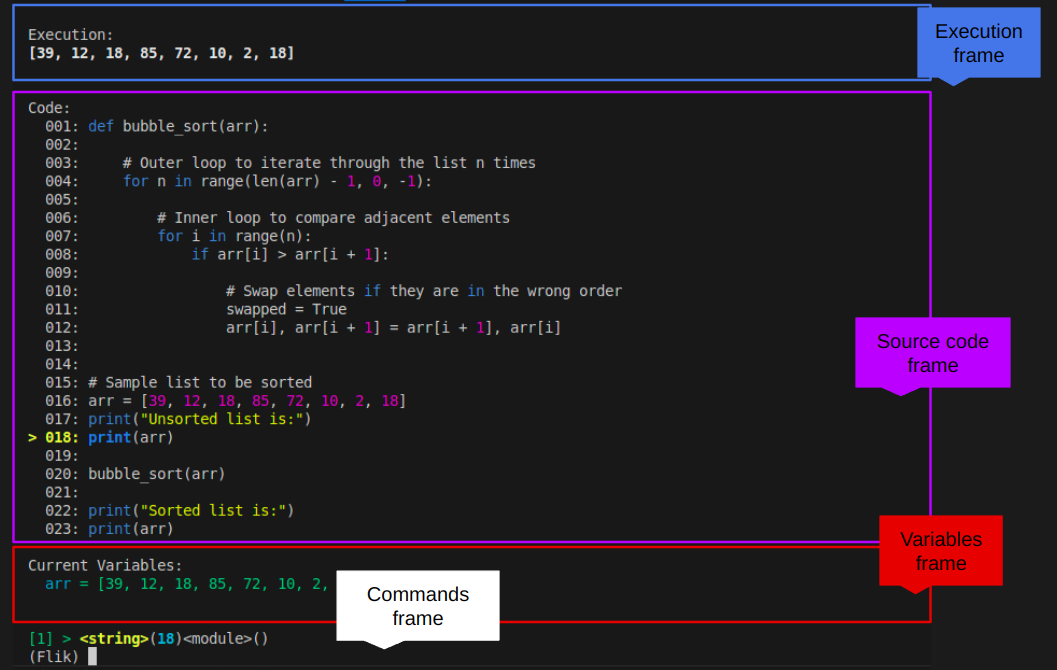
\includegraphics[width=0.9\textwidth]{figures/flik_interface.png}
    \caption{Debugger tool}
    \label{fig:debuggerf}
\end{figure}

% Add example of use step by step. Explain the videos.
We now use a running example to present the features, commands and inner work of \flik. Four 
our running example we use the gridworld \ac{RL} benchmark. The environment consists of a 
$10 \times 10$ grid, shown in \fref{fig:gridworld}. The agent can move in four directions: up, down, 
left, and right at every gridworld cell. However, the movement is not successful in bordering cells 
or cells adjacent to walls (\ie gray-out cells), as it collides with the walls and bounces back to the 
starting position.
The agent's reward is defined obtaining a reward of 1 when the agent gets to the goal state, and a 
reward of -1 when the agent visits trap states, terminating the execution in both cases. The agent 
starts in a fixed position, the top left corner of the grid (the blue state in \fref{fig:gridworld}). 

For the purpose of the running example, we will use the implementation of the gridworld agent shown 
in \fref{lst:gridworld-learner}, explaining the \flik commands used to detect a bug in the code. 
Running the program we pay special attention to the \spy{run} function, which we can access using 
the \spy{n} command until we reach it. Alternatively, it is possible to move directly to a specific 
execution point, by setting breakpoints in the program. For example, when executing the program we 
can use the \spy{c} command to execute until the \spy{breakpoint} in \fref{ln:breakpoint} is reached. 
Once in the function, we use the \spy{n} command to step through the function. 
At particular points in the execution (\eg \fref{ln:stop1}), we can observe variables' values by means 
of the \spy{p} o \spy{pp} commands. In our example, we could use \spy{p self.gamma} to see the 
value of the \spy{gamma} hyperparameter. 

After continuing the execution for a couple of episodes to let the agent train, we can use the 
command \spy{variables}, in \fref{ln:stop2}, to observe the values of the different variables. Upon 
inspection, we have the following observations. First, the historic value of the \spy{action} is $0$ 
throughout the program execution. Second, all values in the \spy{qtable} are unchanged (all continue 
as 0). Third, the value of the \spy{epsilon} hyperparameter is $0.1$. 
Putting both values together, we note that the from the condition in \fref{ln:stop1}, the agent has a 
high probability of tacking the else branch exploiting the known values. However, as the agent has 
not trained updating the values, the exploitation equals to random action choosing, and therefore 
leading to erroneous agent behavior.

\begin{python}[numbers=left,
	caption={\flik running example of the gridworld environment},
	label={lst:gridworld-learner}]
class Agent:
  def __init__(self, env, alpha=0.1, gamma=0.6, epsilon=0.1, episodes=10):
    #hyper parameters
    self.alpha = alpha
    self.gamma = gamma
    self.epsilon = epsilon
    self.environment = env
    self.qtable = self.__initdic__() #initialize q-table
    self.episodes = episodes
    
  def run(self, ui_input):
      done = False
      counter = 0
      breakpoint()  ` \label{ln:breakpoint} `
      for i in range(self.episodes):
        done = False
        while not done:
          current_state = copy.deepcopy(self.environment.state) `\label{ln:back1}`
          if random.uniform(0,1) < self.epsilon:   ` \label{ln:stop1} `
            action = self.random_action(current_state)
          else:
            action = np.argmax(self.qtable[current_state])  
          next_state, reward, done, info = self.step(action) ` \label{ln:stop2} `
          old_value = self.qtable[current_state][action]
          next_max = np.max(self.qtable[next_state])
          new_value = (1-self.alpha)*old_value + self.alpha*(reward+self.gamma*next_max)
          self.qtable[current_state][action] = new_value
          counter += 1
        if ui_input == 1:
          actions, values = self.actions_values()
          self.environment.plot_action(actions, values)
        self.environment.reset()
    return self.qtable
\end{python}

During the execution we can use \flik to confirm that the root cause of the problem is the \spy{epsilon} 
hyperparameter. To do this, from \fref{ln:stop2} we can use the command \spy{back_to 18} to go 
backward in the program execution to \fref{ln:back1}. Then, we can effectively change the value of 
\spy{epsilon} using the \spy{setvar self.epsilon=0.9} command. Once the change is made, if we 
continue execution, after reaching \fref{ln:stop2}, we can print the value of \spy{action} (\spy{p action}), 
to observe now different actions are taken, and the agent can train properly, observing changes for 
values across the q-table. An example of the execution of \flik in the gridworld example is available at: 
\url{https://drive.google.com/file/d/1NyipuWsRr6ZrIbtlvU5qyooHS2aVsWXc/view?usp=sharing}.

\fref{tab:flik-commands}, shows a summary of the commands implemented in \flik, where the 
first six commands in the first block are specific to \flik, and the following 12 commands in the second 
block are provided with \ac{PDB}.

\begin{table}
  \centering
  %\resizebox{\columnwidth}{!}{%
\begin{tabular}{c| p{14.1cm}}
\textbf{Command}               & \multicolumn{1}{c}{\textbf{Description}}  \\ 
\toprule
\spy{step_back} & Goes one step back in time. Moving to the previous line of code from the currently executing line\\
\spy{back_to} & Moves to a program line (in the past) given as parameter, reverting the stack and the program's state according tot he recorded history (\ie loading a previous execution context) \\
\spy{variables} & Shows the local and global variables from the current execution context \\
\spy{args} & Shows the values of the function running right now\\
\spy{setvar} & Modifies the value of a variable (given as parameter) for the current execution context. Note that due to some Python optimizations, and variables' protection this will not work for all variables, but does work for most user-defined variables \\
\spy{sticky} & Returns the debugger mode to \flik if the debugger switches to \ac{PDB} \\
\midrule
\spy{p} & Evaluates and prints the value of the expression given as parameter\\
\spy{pp} & Pretty-prints the value of an expression (after evaluating it) \\
\spy{c} & Continues execution until it stops or it reaches a breakpoint \\
\spy{n} & Continues execution until the next line in the current function, or returns \\
\spy{s} & Executes the current line and stops at the first possible occasion (either in a function that is called or in the current function) \\
\spy{unt} & Continues execution until the line with a greater number than that of the current line is reached. With a line number argument, continues execution until a line with a number greater or equal to the argument is reached \\ 
\spy{b} & Lists all breakpoints when no argument is given. If a line number is given as argument, sets a breakpoint at the given line in the current file, or in a specific file if the \spy{filename:} prefix is used \\
\spy{w} & Prints a stack trace, with the most recent frame at the bottom. An arrow indicates the current frame, which determines the context of most commands \\
\spy{u} & Moves the current frame count one (by default) level up in the stack trace (to an older frame) \\
\spy{d} & Move the current frame count one (by default) level down in the stack trace (to a newer frame) \\
\spy{help} & Shows a list of available commands \\
\spy{q} & Quits the debugger and exits \\
\bottomrule
\end{tabular}%
%}
  \caption{\flik commands description}
  \label{tab:flik-commands}
\end{table}


\endinput


% $Id: evaluation.tex 
% !TEX root = main.tex

\section{Empirical Study}
\label{sec:evaluation}

The purpose of the study was to assess the user experience and usefulness of \flik, when used to detect and locate bugs in  \ac{RL} programs. In particular, the participants were provided with three different RL programs that implement three real-world problems:  (i) GridWorld, (ii) Rooms, and (iii) Cars (Driving assistant). A fault was manually injected in each program, and the task assigned to the participants was to improve the functional quality of the three programs. Note that the injected bugs did not lead the program to exceptions or crashes, i.e., each program ran and there was no evident buggy behavior. The injected bugs made the programs to generate outputs that do not match the expected outputs. Concerning the participants, master students from the Reinforcement Learning course at Universidad de los Andes were recruited.  The participants were provided with a evaluation  \fref{sec:eval-guide}, that describes the purpose of the tool, the task and steps, instructions on how to run and 
use the tool, documentation of the tool, and an small example. The real-world problems implemented for the study are described as follows:



%To evaluate and validate \flik as a framework to support the development of \ac{RL} programs, and in consequence to help increase their quality, an initial empirical evaluation was conducted. The evaluation consists of three different test scenarios  from real-world problems that arise in the development of \ac{RL} programs, and the evaluation aimed

%The purpose of the evaluation is to observe three scenarios: gridwrold, rooms and cars that cover from  the creation of an \ac{RL} program from scratch to the process of optimizing learning parameters, aiming to determine the specific values to start with to achieve the most optimal convergence for the program. In each of the programs a bug is added ensuring strange application behavior, but ensuring the application to run, therefore, the expected output does not match the real output of the programs. The intention of the evaluation scenarios is to if \flik can actually improve the performance and development of \ac{RL} %programs.

%The empirical evaluation is performed with a group of students from the \ac{RL} course at Universidad de  los Andes. We attached the evaluation guide given to the students in \fref{sec:eval-guide}, in which  is described the purpose of the tool, the description of the activity with the steps on how to run and  use the tool, a small documentation of the tool, and an small example.

%\subsection{Exercise 1: GridWorld}
%\label{sec:grid-eval}
\vspace{0.3cm}
\textbf{GridWorld}. This environment consists of a $n \times n$ ($10\times 10$ in our example) rectangular  board/grid, in which each tile $(i,j)$ represents a specific state of the board. Tiles in the board may be  walls, which agents cannot cross. Additionally, there are special exit  tiles that give a positive or negative reward to agents, as shown in \fref{fig:gridworld}. All tile types are unknown to the agent that moves from a given starting point in the board, searching for the goal state (\ie exit states with positive reward of $1$). The agent moves from state to state, avoiding  obstacles and incorrect exit states (which give a reward of $-1$ when used to exit). 

The program has a bug for the $\epsilon$ parameter, presenting an error in the probability which defines which action is taken next. This introduces a wrong behavior for the \ac{RL} 
agent because $\epsilon$ will be so small that only in the first iteration the action will be taken randomly and in the follow iterations the probability will be so small to take another action that the agent will not explore other action policies. This is an undesired behavior specially for training purposes as an agent should have a large probability to choose other actions and explore the grid. The idea in this task is that the study participants use \flik to navigate through the code and find out why the agent is not learning properly. And eventually, the participants should come out with the solution of increasing the value of $\epsilon$. 

\begin{figure}[h]
  \centering
  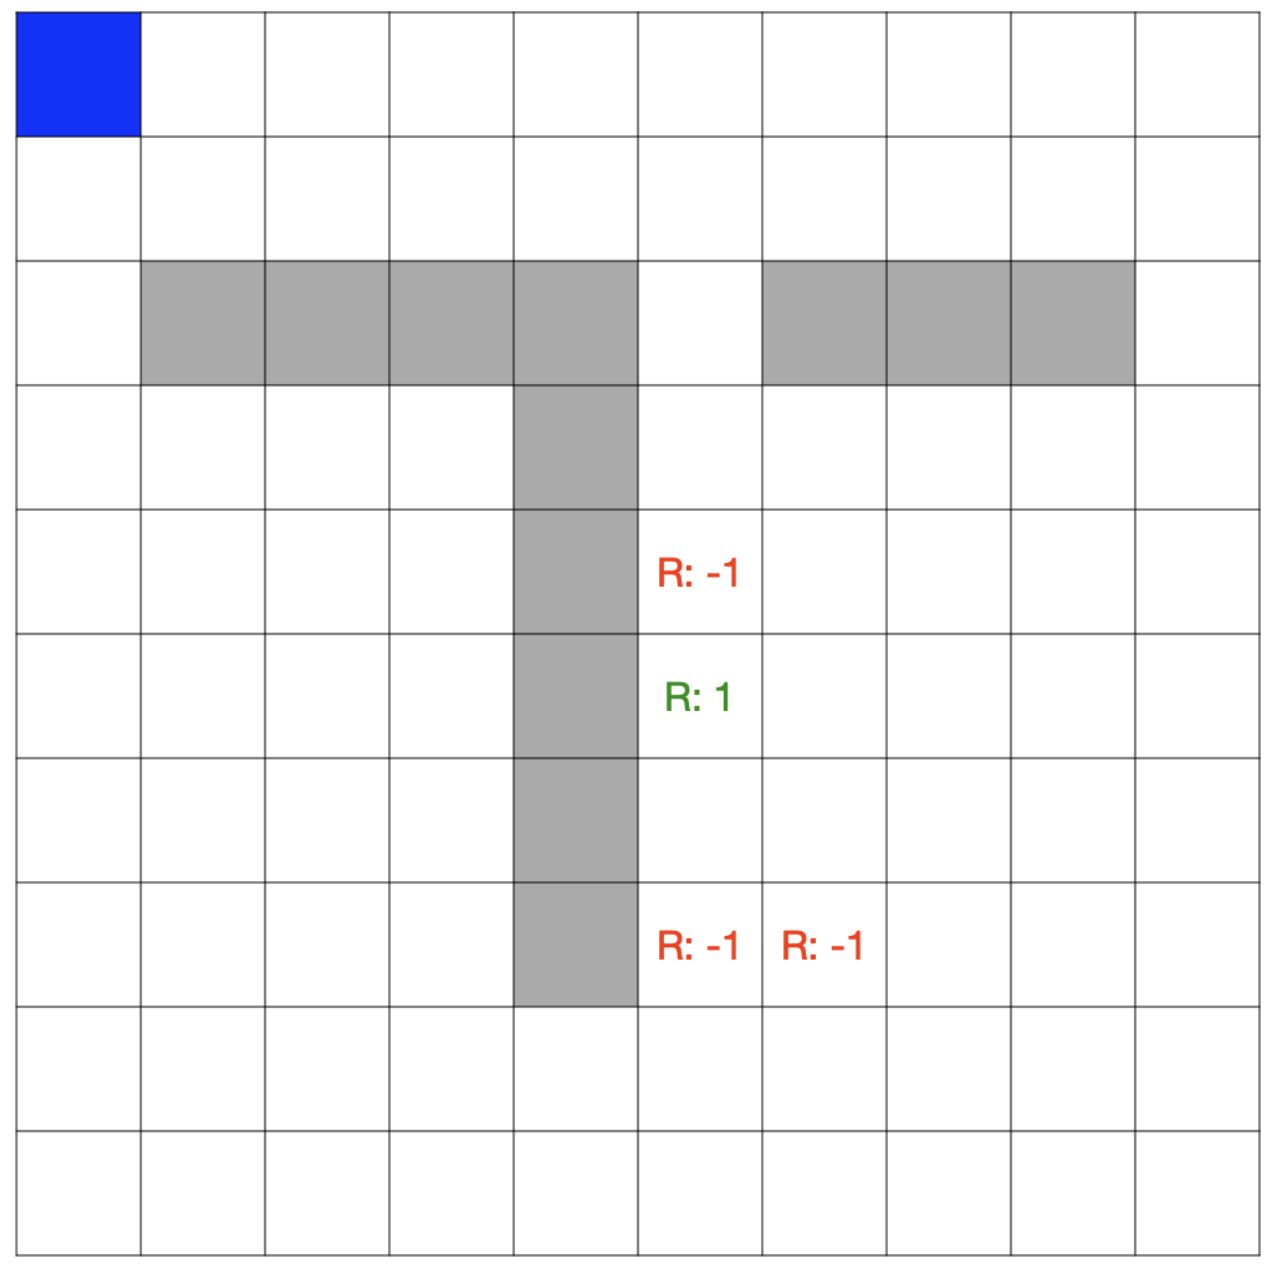
\includegraphics[width=0.5\columnwidth]{figures/gridworld.png}
  \caption{10x10 gridworld environment example}
  \label{fig:gridworld}
\end{figure}



%\subsection{Exercise 2: Rooms}
%\label{sec:rooms-eval}

\textbf{Rooms.} The four rooms maze environment consists of a $13\times 13$ board/grid divided in $4$ sections 
(\ie rooms), with walls between them, and a door opening to go from one room to another, as shown 
in \fref{fig:rooms}. The agent's objective in this environment is to exit through the upper-left room 
(the green square) in the fewest possible steps. Reaching the exit state gives a reward of $1$, and no 
other action give a reward to the agent. In each episode the agent starts from any valid position in the 
grid, \eg the yellow square in the bottom-right room in the figure. 

\begin{figure}[h]
  \centering
  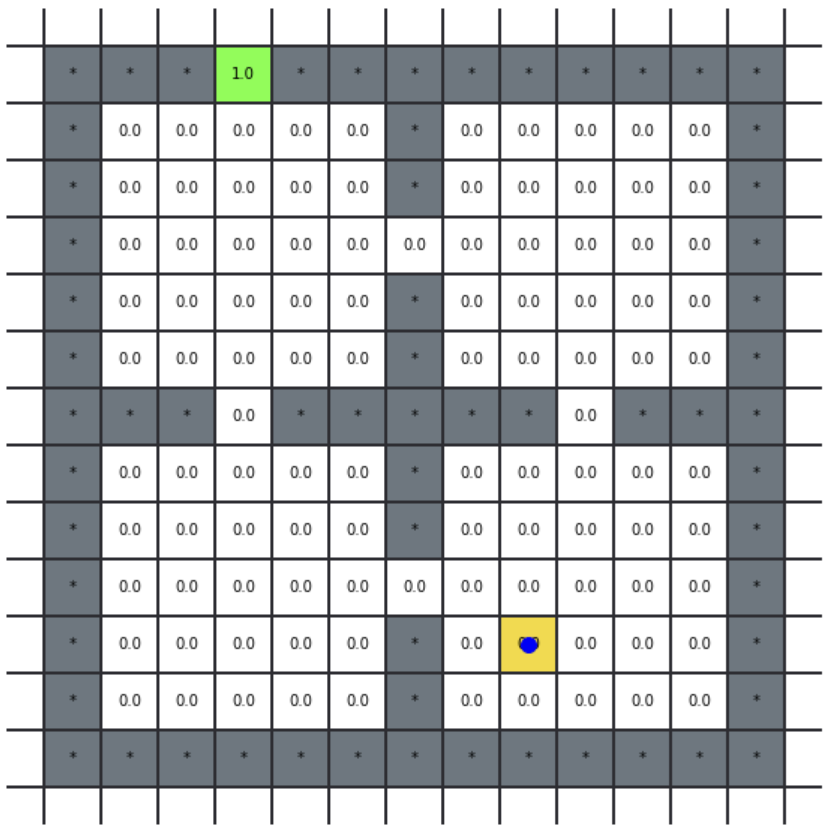
\includegraphics[width=0.5\columnwidth]{figures/rooms.png}
  \caption{Rooms environment example with associated rewards in each state}
  \label{fig:rooms}
\end{figure}

In the program, we introduced a bug in the learning rate $\alpha$, on the Q-learning equation, thus,  the original values for the learning rate alpha are exchanged like:

\begin{itemize}
\item Original equation:
$
Q(s, a) \leftarrow (1-\alpha) Q(s, a) + \alpha \left( r + \gamma \max_{a'} Q(s', a') \right)
$

\item Wrong equation to debug:
$
Q(s, a) \leftarrow  \alpha Q(s, a) + (1-\alpha) \left( r + \gamma \max_{a'} Q(s', a') \right)
$
\end{itemize}

In the original equation,  $(1-\alpha) Q(s, a)$ is the current value and $\gamma \max_{a'} Q(s', a')$ 
the maximum reward that can be obtained from state $s'$. This means that if the learning rate is very 
small the current value will keep almost the same, turning a little bit towards the reward and the 
maximum value given the action; this will make that the agent learn short steps towards the 
optimal policy. In the Q-learning formula, the learning rate $\alpha$ defines how much the old estimate $Q(s,a)$ 
is revised based on the new information. It ensures that over time, the algorithm balances past 
knowledge with current learning, gradually incorporating new information while retaining important 
aspects of previous learning. Changing the equation in this way will disrupt this balance. Specifically,
$(1-\alpha)$ scales the difference between the new estimate and the old estimate. This makes the new information less influential as $\alpha$ gets larger, while the old value gets re-scaled by $\alpha$,  which does not align with the expected behavior of a Q-learning update. The idea in this task is that the participants use \flik to navigate through the code and find out the reason why the agent is not learning properly, afterwards we expected the participant to figure out a solution adjusting the proper value to update the Q-Learning equation.

%\subsection{Exercise 3: Driving Assistant}
%\label{sec:cars-eval}
\textbf{Cars (Driving Assistant)}. In this case the agent must learn to drive, on the correct lane, at the allowed speed, taking over slow traffic, and not crashing. The possible actions for the agent are: straight, slow\_down, speed\_up, steer\_left, steer\_right. Figure \ref{fig:cars-code-example} depicts the visual interface of this environment.

\begin{figure}[h]
    \centering
    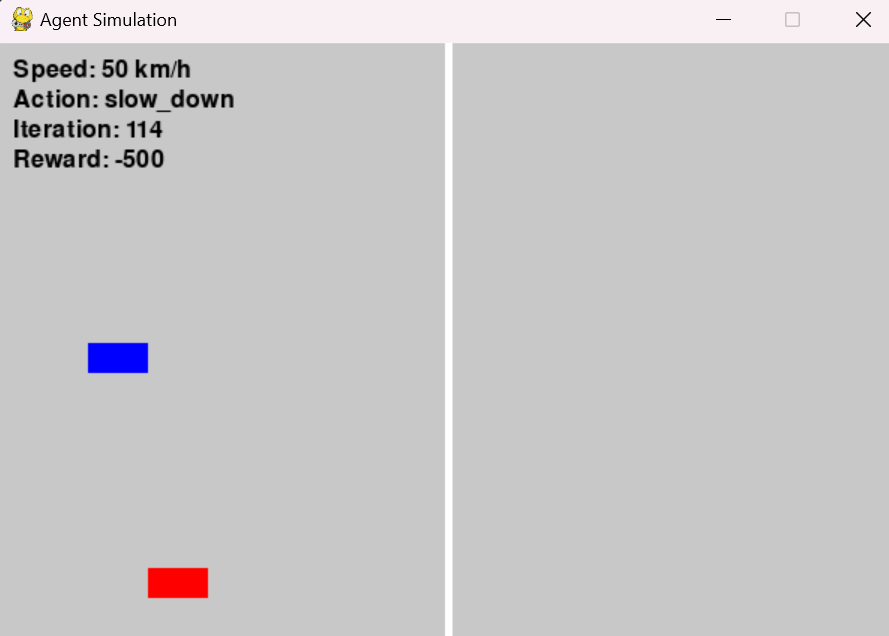
\includegraphics[width=0.5\textwidth]{figures/cars_example.png}
    \caption{Cars code example}
    \label{fig:cars-code-example}
\end{figure}

This is the largest task for the participants to analyze with \flik. % and see why the agent was not learningcorrectly, with respect to the expected. 
The bug introduced in this application is in the reward function, not motivating the agent to drive at the speed limit. The policy learned by the agent emerges as stopping or go very slow, which is not the expected behavior. Through exploration using \flik, developers are expected to observe the behavior of the reward and update it so that the agent can learn to drive appropriately.
as expected.

%% Add way of evaluation, explanation about the survey, questions.
%\subsection{Evaluation setup}
%\label{sec:evaluation}

For the user evaluation we had a session with 27 developers (\ie graduate students). 
The developers were asked to complete the three tasks (\ie gridworld, rooms, cars) described previously. The full evaluation session used a time-slot of 1h30 split as follows 
\begin{enumerate}[label=(\arabic*)]
\item During the first 15 minutes the tool and a usage example were presented to the participants; (shown in \fref{sec:eval-guide}).
\item 50 minutes to complete the tasks; 15 minutes to finish the first task, 15 minutes to finish the second task, and  20 minutes to finish the third task. 
\item At the end of the session, the students were asked to fill an evaluation survey 
\end{enumerate}

The evaluation survey, defined as a google form, is divided in three sections: general knowledge questions, task questions, and usability.
The general knowledge questions were about the participants' experience  using Python, debuggers and  terminal. The task questions were about the bug encountered in each of the tasks, and how the the bug was fixed (if fixed). The usability  questions were regarding the participants experience with the debugger usability, and additional feedback they could provide for improving \flik. The survey was anonymized, and the questions were inspired by the 
back in time debugger for JavaScript study~\cite{leger23}, and the responses are available 
at \url{https://shorturl.at/DhN56}. 

The survey had 23 multiple choice questions with a 5-points Likert scale,  in which 5 meant completely agreed, and 1 meant completely disagreed. One of the questions was a yes or no answer, to identify if the students wanted to use the tool in the future. Finally, there were 10 open-answer questions , to dive deeper into feedback for the tool, and the tasks' complexity.


%Finally, there are two examples of the tool being used. In the first  example, the tool is used to debug a simple program, this was used to introduced to the students  the simple commands they could use like stepping (forward and backwards), modifying, or inspecting variables. In the second example, the tool is used to debug a \ac{RL} program, specially the gridworld example. The link to find this videos is: \url{https://shorturl.at/rD343} 



\endinput


% $Id: results.tex 
% !TEX root = ../main.tex

\section{Analysis and Results}
\label{sec:results}

This section presents the analysis of the results of the empirical study presented in 
\fref{sec:evaluation}. The results are presented according to three sections in the survey: General 
knowledge (\fref{sec:general-knowledge}), Task Effectiveness (\fref{sec:tasks-results}) and usability 
(\fref{sec:usability}). Additionally, a discussion section is added analyzing the results form the survey. 
All data obtained from the evaluation is available as part of the data and replication 
package.\footnote{available at: \url{https://github.com/larodriguez22/Flik_Experiments}} 


%%
\subsection{General Knowledge Results}
\label{sec:general-knowledge}

Most of the participants were very experienced with programming in Python as it can be seen in 
(\fref{fig:python-experience}). The experience level of 5 is selected as participants use Python very 
often in their work and university courses. 
Similarly, most participants are well familiarized with \ac{RL} (\fref{fig:rl-experience}), as they were 
taking a course on the topic. This is very important information, as the bugs required familiarity with 
\ac{RL} and Python knowledge to be identified. Furthermore, the participants report being familiar 
with using the terminal, and therefore, interacting with \flik, using the commands and the interface 
would not pose a problem or require a learning curve (\fref{fig:terminal-experience}). 
Nevertheless, in average, the participants were not familiarized with debuggers, and only used them  
rarely, normally using Visual Studio Code interface's simple features, like graphical breakpoint 
functionality. This lead to misunderstandings and some difficulties in completing the tasks, as the 
tool is based on command line interaction to stop and step through the code 
(\fref{fig:debugging-experience}). This characteristic from the participants caused a steeper learning 
curve to use the tool, than expected from participants with previous debugger experience.

In all the graphs in \fref{fig:general-know} the y-axis represents the number of participant  
responses for each question for a particular score in the Likert scale, and the x-axis represents score, 
between 5 and 1 (from completely agree to completely disagree).

\begin{figure}[hptb]
    \centering
    \begin{subfigure}[b]{0.45\textwidth}
        \centering
        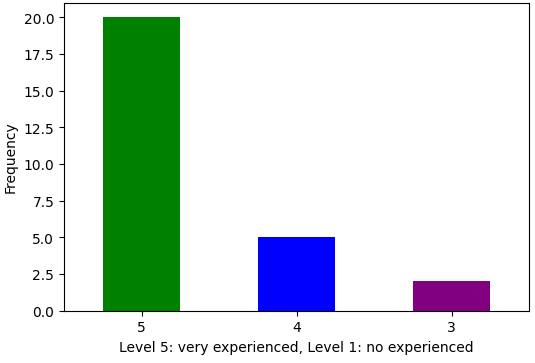
\includegraphics[width=\textwidth]{figures/experience-python}
        \caption{Experience using Python}
        \label{fig:python-experience}
    \end{subfigure}
    ~ 
    \begin{subfigure}[b]{0.45\textwidth}
        \centering
        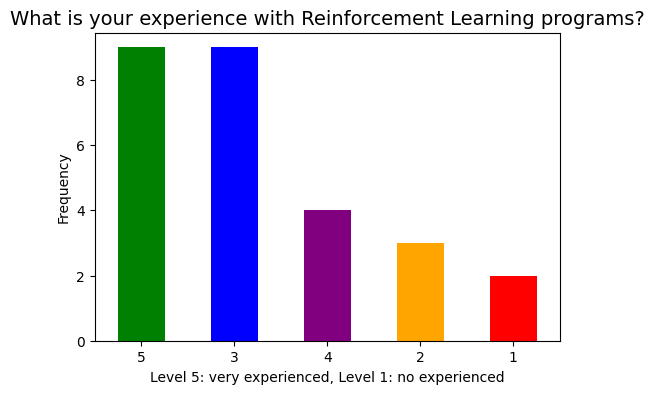
\includegraphics[width=\textwidth]{figures/experience-rl}
        \caption{Experience in \ac{RL}}
        \label{fig:rl-experience}
    \end{subfigure}
    ~ 
    \begin{subfigure}[b]{0.45\textwidth}
        \centering
        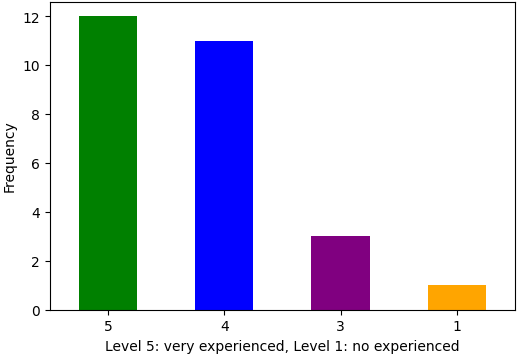
\includegraphics[width=\textwidth]{figures/experience-terminal}
        \caption{Experience using the terminal}
        \label{fig:terminal-experience}
    \end{subfigure}
    ~ 
    \begin{subfigure}[b]{0.45\textwidth}
        \centering
        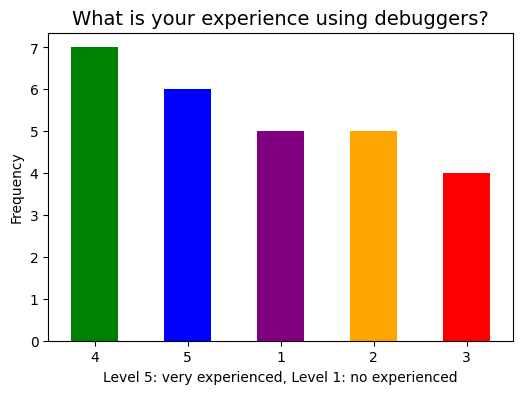
\includegraphics[width=\textwidth]{figures/experience-debuggers}
        \caption{Experience in debugging}
        \label{fig:debugging-experience}
    \end{subfigure}
    \caption{Experience reported by users in the four main dimensions of the tools used in the evaluation}
    \label{fig:general-know}
\end{figure}


%%
\subsection{Tasks Results}
\label{sec:tasks-results}

Taking the results reported from the three tasks, most of the participants completed the first task 
successfully (\fref{fig:task1}). Participants reported the task was easy to solve. Even though the task 
was reported to be easy, it took participants a long time to complete, because this was the task in 
which participants had to get familiarized with the tool. The second task was harder than the first one, 
as participant were not familiar with the problem, and its complexity is higher. Most participants took 
longer to finish task2 (\fref{fig:task2}), and struggled finding the root cause of the bug in the program. 
Such result is expected, as the bug introduced in task 2, does not exhibit a completely wrong agent 
behavior, but a more subtle interaction with the environment and the obtained Q-values. Moreover, the 
fix required more than updating a value, but actually modifying the learning function. Such required 
changed confused many of participants. Finally, the third task (\fref{fig:task3}) was the hardest 
task, most participants had trouble finding the bug. The general comments about the task is that it 
was not easy to solve. Nevertheless, the participants managed to finish the task in less time than in 
the other tasks. 

From the results it is expected that identifying and fixing the bug in the first task take longer than for 
other tasks, even though this is the easiest task, participants are still getting familiarized with the tool, 
and the learning curve for debugging the programs is steep. In the following tasks, while the nature of 
the introduced bugs is different, there is a learning curve  with using the tool. For the second task,
given the nature of the bug and the fact that the bug was introduced in the Q-learning algorithm's 
logic, it was harder to identify. Hence, this task was harder to solve, even though was completed by 
most participants. Finally, for the third task, the introduced bug had yet a different nature, in the 
reward function. For this tasks the learning curve in using the tool was more developed, and it took 
participants less time than expected for this reason.

In \fref{fig:general-know} the y-axis represents the number of participants registering 
answers to the question at the given Likert score. The x-axis corresponds to the score, with
values in the range from 5 to 1 (from completely agree, to completely disagree). In the last 
question (the third bar in green for all graphs), 5 represents taking a lot of time, and 1 represents 
taking very little time.

\begin{figure}[hptb]
    \centering
    \begin{subfigure}[b]{0.32\textwidth}
        \centering
        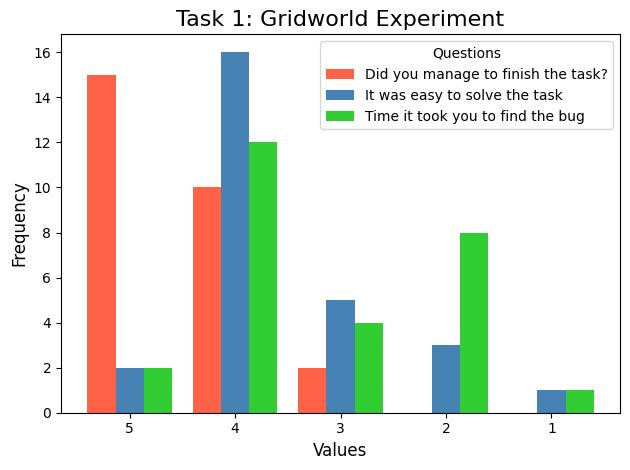
\includegraphics[width=\textwidth]{figures/task1}
        \caption{Gridworld task}
        \label{fig:task1}
    \end{subfigure}
    ~ 
    \begin{subfigure}[b]{0.32\textwidth}
        \centering
        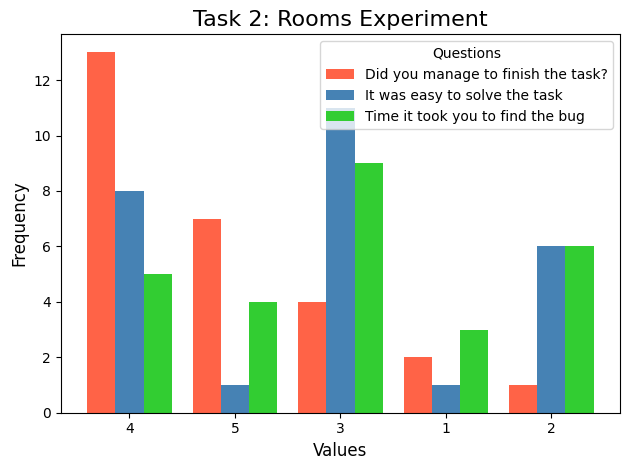
\includegraphics[width=\textwidth]{figures/task2}
        \caption{Rooms task}
        \label{fig:task2}
    \end{subfigure}
    ~ 
    \begin{subfigure}[b]{0.32\textwidth}
        \centering
        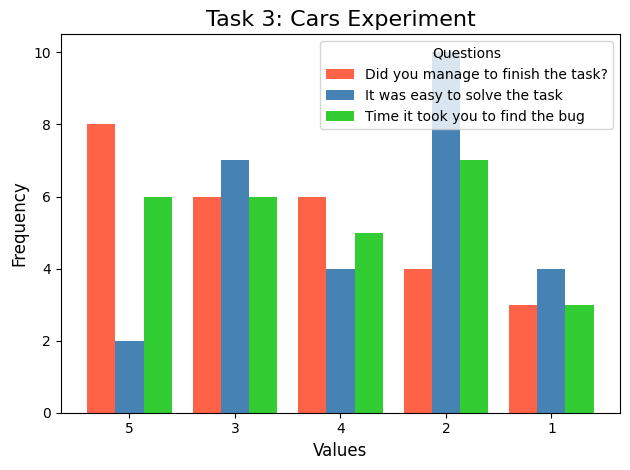
\includegraphics[width=\textwidth]{figures/task3}
        \caption{Cars task}
        \label{fig:task3}
    \end{subfigure}
    \caption{Results of the tasks to solve}
    \label{fig:general-know}
\end{figure}


%%
\subsection{Debugger Usability Results}
\label{sec:usability}

The results for  the debugger's usability, shown in \fref{tab:general1-debuggers} and 
\fref{tab:general2-debuggers}, exhibit a sense that the tool is useful. The comments, in general,  
express that \flik would be useful, specially if given more time to study it, and gain practice with the 
tool before using it in real tasks. The tool was easy to use, once familiarized with the commands and 
their use. Additionally, there are several comments about providing a GUI or improving the current UI,
to help understanding how the tool works, and how to navigate the code with it, as at it differs from 
more mainstream debuggers like the one available with Visual Studio Code and its interface.

\begin{table}[H]
  \centering
  \caption{General Results Part 1}
  \resizebox{\columnwidth}{!}{%
\begin{tabular}{c | *{5}{>{\centering\arraybackslash}p{5cm}}} 
  & \textbf{I have found too much inconsistency in this system} 
  & \textbf{I think most people would learn to use the system quickly} 
  & \textbf{I found the system quite awkward to use} 
  & \textbf{I have felt very safe using the system} 
  & \textbf{I would need to learn a lot of things before I could handle the system} \\
\toprule
\textbf{5} & {1}   & {7}  & {4}  & {7}   & {8.0}                                                                                                                        \\
\textbf{4} & {2}                                                                                                      & {6}                                                                                                             & {7}                                                                                           & {8}                                                                                          & {6.0}                                                                                                                        \\
\textbf{3} & {4}                                                                                                      & {6}                                                                                                             & {9}                                                                                           & {7}                                                                                          & {4.0}                                                                                                                        \\
\textbf{2} & {7}                                                                                                      & {6}                                                                                                             & {4}                                                                                           & {4}                                                                                          & {0.0}                                                                                                                        \\
\textbf{1} & {13}                                                                                                     & {2}                                                                                                             & {3}                                                                                           & {1}                                                                                          & {9.0}                                                                                                                       
\end{tabular}%
}

  \label{tab:general1-debuggers}
\end{table}

\begin{table}[H]
  \centering
  \caption{General Results Part 2}
  \resizebox{\columnwidth}{!}{%
\begin{tabular}{ c |  *{5}{>{\centering\arraybackslash}p{4cm}}}
% \multicolumn{6}{c}{\cellcolor[HTML]{FFFFFF}{ \textbf{Task 2: Rooms Experiment.}}}                                                                                                                                                                                                                                                                                                                                                                                                                                                                                                                                                                                      \\
 & \textbf{I think I would like to use this system frequently} 
 & \textbf{I find this system unnecessarily complex}
 & \textbf{I think the system is easy to use}
 & \textbf{I think I would need technical support to use the system} 
 & \textbf{I find the various functions of the system quite well integrated} \\
 \toprule
\textbf{5} & { 7}                                                                                                      & { 2}                                                                                            & { 5}                                                                                   & { 9}                                                                                                            & { 6}                                                                                                                    \\
\textbf{4} & { 5}                                                                                                      & { 7}                                                                                            & { 5}                                                                                   & { 8}                                                                                                            & { 13}                                                                                                                   \\
\textbf{3} & { 7}                                                                                                      & { 7}                                                                                            & { 11}                                                                                  & { 4}                                                                                                            & { 5}                                                                                                                    \\
\textbf{2} & { 7}                                                                                                      & { 6}                                                                                            & { 6}                                                                                   & { 3}                                                                                                            & { 2}                                                                                                                    \\
\textbf{1} & { 1}                                                                                                      & { 5}                                                                                            & { 0}                                                                                   & { 3}                                                                                                            & { 1}                                                                                                                   
\end{tabular}%
}

  \label{tab:general2-debuggers}
\end{table}

% \begin{table}[]
% \centering
%  \resizebox{\columnwidth}{!}{%
 \begin{tabular}{ c | *{5}{>{\centering\arraybackslash}p{3cm}}}
 \multicolumn{11}{c}{\cellcolor[HTML]{FFFFFF}{ \textbf{Debugger Usability.}}}                                                                                                                                                                                                                                                                                                                                                                                                                                                                                                                                                                                                                                                                                                                                                                                                                                                                                                                                                                                                                                                                                                                                                                                                                                                         \\
 { \textbf{}}  & { \textbf{\begin{tabular}[c]{@{}c@{}}I think I would like to use this \\ system frequently\end{tabular}}} & { \textbf{\begin{tabular}[c]{@{}c@{}}I find this system \\ unnecessarily complex\end{tabular}}} & { \textbf{\begin{tabular}[c]{@{}c@{}}I think the system \\ is easy to use\end{tabular}}} & { \textbf{\begin{tabular}[c]{@{}c@{}}I think I would need technical \\ support to use the system\end{tabular}}} & { \textbf{\begin{tabular}[c]{@{}c@{}}I find the various functions of the \\ system quite well integrated\end{tabular}}} & { \textbf{\begin{tabular}[c]{@{}c@{}}I have found too much \\ inconsistency in this system\end{tabular}}} & { \textbf{\begin{tabular}[c]{@{}c@{}}I think most people would learn \\ to use the system quickly\end{tabular}}} & { \textbf{\begin{tabular}[c]{@{}c@{}}I found the system quite \\ awkward to use\end{tabular}}} & { \textbf{\begin{tabular}[c]{@{}c@{}}I have felt very safe \\ using the system\end{tabular}}} & { \textbf{\begin{tabular}[c]{@{}c@{}}I would need to learn a lot \\ of things before I could handle the system\end{tabular}}} \\
 { \textbf{5}} & { 7}                                                                                                      & { 2}                                                                                            & { 5.0}                                                                                   & { 9}                                                                                                            & { 6}                                                                                                                    & { 1}                                                                                                      & { 7}                                                                                                             & { 4}                                                                                           & { 7}                                                                                          & { 8.0}                                                                                                                        \\
 { \textbf{2}} & { 7}                                                                                                      & { 6}                                                                                            & { 6.0}                                                                                   & { 3}                                                                                                            & { 2}                                                                                                                    & { 7}                                                                                                      & { 6}                                                                                                             & { 4}                                                                                           & { 4}                                                                                          & { 0.0}                                                                                                                        \\
 { \textbf{3}} & { 7}                                                                                                      & { 7}                                                                                            & { 11.0}                                                                                  & { 4}                                                                                                            & { 5}                                                                                                                    & { 4}                                                                                                      & { 6}                                                                                                             & { 9}                                                                                           & { 7}                                                                                          & { 4.0}                                                                                                                        \\
 { \textbf{4}} & { 5}                                                                                                      & { 7}                                                                                            & { 5.0}                                                                                   & { 8}                                                                                                            & { 13}                                                                                                                   & { 2}                                                                                                      & { 6}                                                                                                             & { 7}                                                                                           & { 8}                                                                                          & { 6.0}                                                                                                                        \\
 { \textbf{1}} & { 1}                                                                                                      & { 5}                                                                                            & { 0.0}                                                                                   & { 3}                                                                                                            & { 1}                                                                                                                    & { 13}                                                                                                     & { 2}                                                                                                             & { 3}                                                                                           & { 1}                                                                                          & { 9.0}                                                                                                                       
 \end{tabular}%
 }

% \end{table}

In Tables \ref{tab:general1-debuggers} and \ref{tab:general2-debuggers} the scale represents the 
Likert score option, expressing whether the participants completely agree ($5$) or completely disagree 
($1$) with he question at hand. The values inside the tables correspond to the number of participants 
that reported each given scale.

%%
\subsection{Discussion}
\label{sec:discussion}

In general, the results of the empirical evaluation are very positive. Most of the participants have a 
good impression of \flik, finding it to be useful, specially for the kind of challenges presented in 
\ac{RL} programs. While participants found it hard to familiarize themselves with the tool, specially 
for the participants with little experience with debuggers, at the beginning at the evaluation session, 
most of the participants found the tool easy to use (after some initial use). Additionally, participants 
mention the tool be of use in general for the development of \ac{RL} programs in general, for example 
to develop course work, identifying the errors in the study as recurrent during development. the 
participants to the empirical study highlight \textbf{\flik is useful in detecting common and hard to 
identify errors and miss behavior in \ac{RL} programs}.

With respect to the usability dimension the participants reported that, with some difficulties at the 
beginning, again for the participants without previous experience with debuggers, 
\textbf{\flik is usable}. The usability of the tool is confirmed by the completion of the three tasks by a 
majority of the participants, and the rapid learning curve gathered when switching between tasks, 
reaching a faster and more fluent code navigation to inspect the program, identify the cause of the 
error, and fix the bug, as reported in the time taken to complete each task. Nonetheless, the 
participants note that to increase the usability of \flik \textit{it is desirable to implement more GUI 
features closer to common features used in other debuggers, as the Visual Studio Code debugger}.


\endinput


% $Id: conclusion.tex 
% !TEX root = ../main.tex

\section{Conclusion and Future Work}
\label{sec:conclusion}

In this work, we presented \flik, a back-in-time debugger for \ac{RL} programs. The introduction of \flik 
is motivated by problems detected in \ac{RL} systems development. First, \ac{RL} programs are 
complex in terms of the interaction between the agent and the environment. Second, the computational 
complexity of the environments come with high costs of training and retraining agents whenever 
unexpected behavior is observed. 
In the former case, understanding the behavior of agents becomes more difficult for developers, as this 
comes from the interaction itself and the valuation associated with each interaction, not just the 
sequence of program instructions to follow. In the latter case, developers must unwind long iterative 
execution traces for the different episodes to identify the location or cause of the strange behavior, 
which for small \ac{RL} programs can already have over thousands of iterations. Continuously training 
the agents for debugging can be very time-consuming and use significant computational resources.

A back-in-time debugger strategy is beneficial for the scenario of \ac{RL} programs as it lets 
developers to interact with their agents directly, not just as a postmortem activity, enabling the 
opportunity to go back in the execution of a program, recover all of its state and context of execution, 
update the system's state, and observe the effect of the agent with respect to the changed state, 
generating a new execution path, without the need to stop or completely retrain agents. These features 
are desirable to tackle the problem of interaction and long execution of \ac{RL} programs. Our proposed 
debugger enables developers to inspect the state of the program in terms of variables, additionally 
providing a functionality to interact with the execution of the program going forward and backwards.

We validate a back-in-time debugger is indeed useful to identify the root cause of bugs through an 
empirical study where 27 participants used \flik in the identification of bugs for three different \ac{RL} 
programs. Most study participants managed to understand the behavior of the agent and find the root 
cause of the bug for the three programs. Specifically, \flik proved  to be useful to find general bugs that 
an \ac{RL} program can present during development. 
Additionally, in the study we evaluated the usability of \flik as a debugging. Even though \flik is a 
console-based debugger, it allows developers to interact with a program during its execution, inspect 
the internal state of the agent, and modify its state and behavior in real-time. 

There are three important avenues of future work to improve the usability of \flik, as gathered from the 
empirical study and the development process. 

First, we want to optimize memory consumption by using layer cashing using a similar strategy to that 
used in git or docker, as a means to save states. Instead of saving the entire history of all variables 
(global and local), and all the metadata of the program for each execution point, we could 
save the changes made on the program since the last recorded history. This would optimize the 
memory usage of \flik. We envision such a change to require a more complex logic and evolving the 
design of \flik to an architecture to support the new features. 

Second, we can develop a full visual interface for \flik, following similar debugger interfaces (\eg 
VSCode or Eclipse) as plugins to an IDE. In this way developers could easier interact with the features 
(commands) of the debugger in a more friendly way. This for example, would also open the opportunity 
to generate visualization for the different execution traces from the re-execution of parts of the program.
Improving the interface of \flik could reduce the complexity of understanding \ac{RL} program,
making it easier to navigate the code and jump back in time.

Finally, \flik could be improved by integrating visualization environments and graphs, as created with 
matplotlib or pygame, so the user could have a better understanding of the environment and the 
agent's behavior, while debugging the program.


\endinput


%%
% !TEX root = ../main.tex
\bibliographystyle{cas-model2-names}
%\biboptions{sort&compress}
\bibliography{local,bib/general, bib/compsci, bib/learning, bib/strings}
%\printbibliography


\end{document}


\endinput

